\section{Digitální chodbové termostaty}
\label{sec:digitalni-chodbove-termostaty}
\begin{figure}[H]
   \centering
   \def\svgwidth{0.4\columnwidth}
   \input{images/svg/otopna-soustava/vyrez-lokalni-termostaty.pdf_tex}
    \caption[Umístění chodbových termostatů.]{Výřez z obrázku \ref{fig:otopna-soustava-a-elektronika-rez-domu}. Umístění chodbových termostatů.}
    \label{fig:vyrez-lokalni-termostaty}
\end{figure}

Na obrázku \ref{fig:vyrez-lokalni-termostaty} je výřez části z celkového nákresu (obrázek \ref{fig:otopna-soustava-a-elektronika-rez-domu}) systému znázorňující umístění chodbových termostatů. Pro snímání teplot z jednotlivých pater na chodbách slouží zakoupené digitální termostaty s označením W3230. Termostat disponuje jedním spínací výstupem (v případě potřeby vytápění se výstup sepne, jinak je rozepnut). Je možné nastavit hysterezi, časové zpoždění, kalibraci teploty a rozsah maximálních teplot. Lze také aktivovat signalizaci, která se spustí po dosažení maximální přípustné teploty. Pro napájení je potřeba stejnosměrné napětí 12 V. Pro snímání teploty slouží NTC termistor. Rozsah teplot je -40 °C až 120 °C. Přesnost měření je $\pm$ 0,1 °C. Termostat lze nahradit za jakýkoliv jiný, který disponuje spínacím výstupem.


\begin{figure}[H]
    \centering
    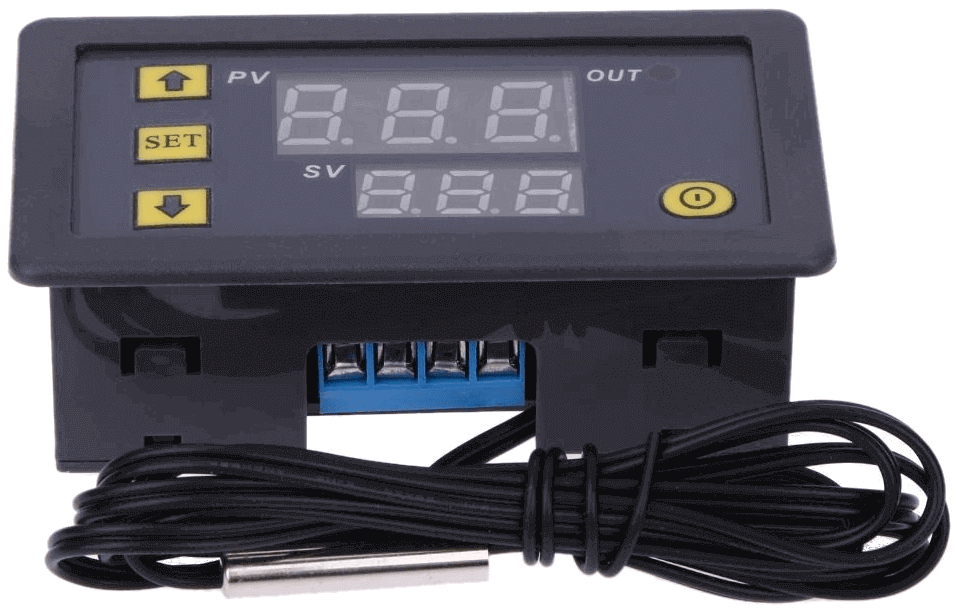
\includegraphics[width=0.5\textwidth]{images/digitalni-termostat-w3230.png}
    \caption[Digitální chodbový termostat W3230.]{Digitální chodbový termostat W3230 \cite{digitalni-termostat-w3230}.}
    \label{fig:digitalni-termostat-w3230}
\end{figure}